\begin{figure}[H]
    \centering
    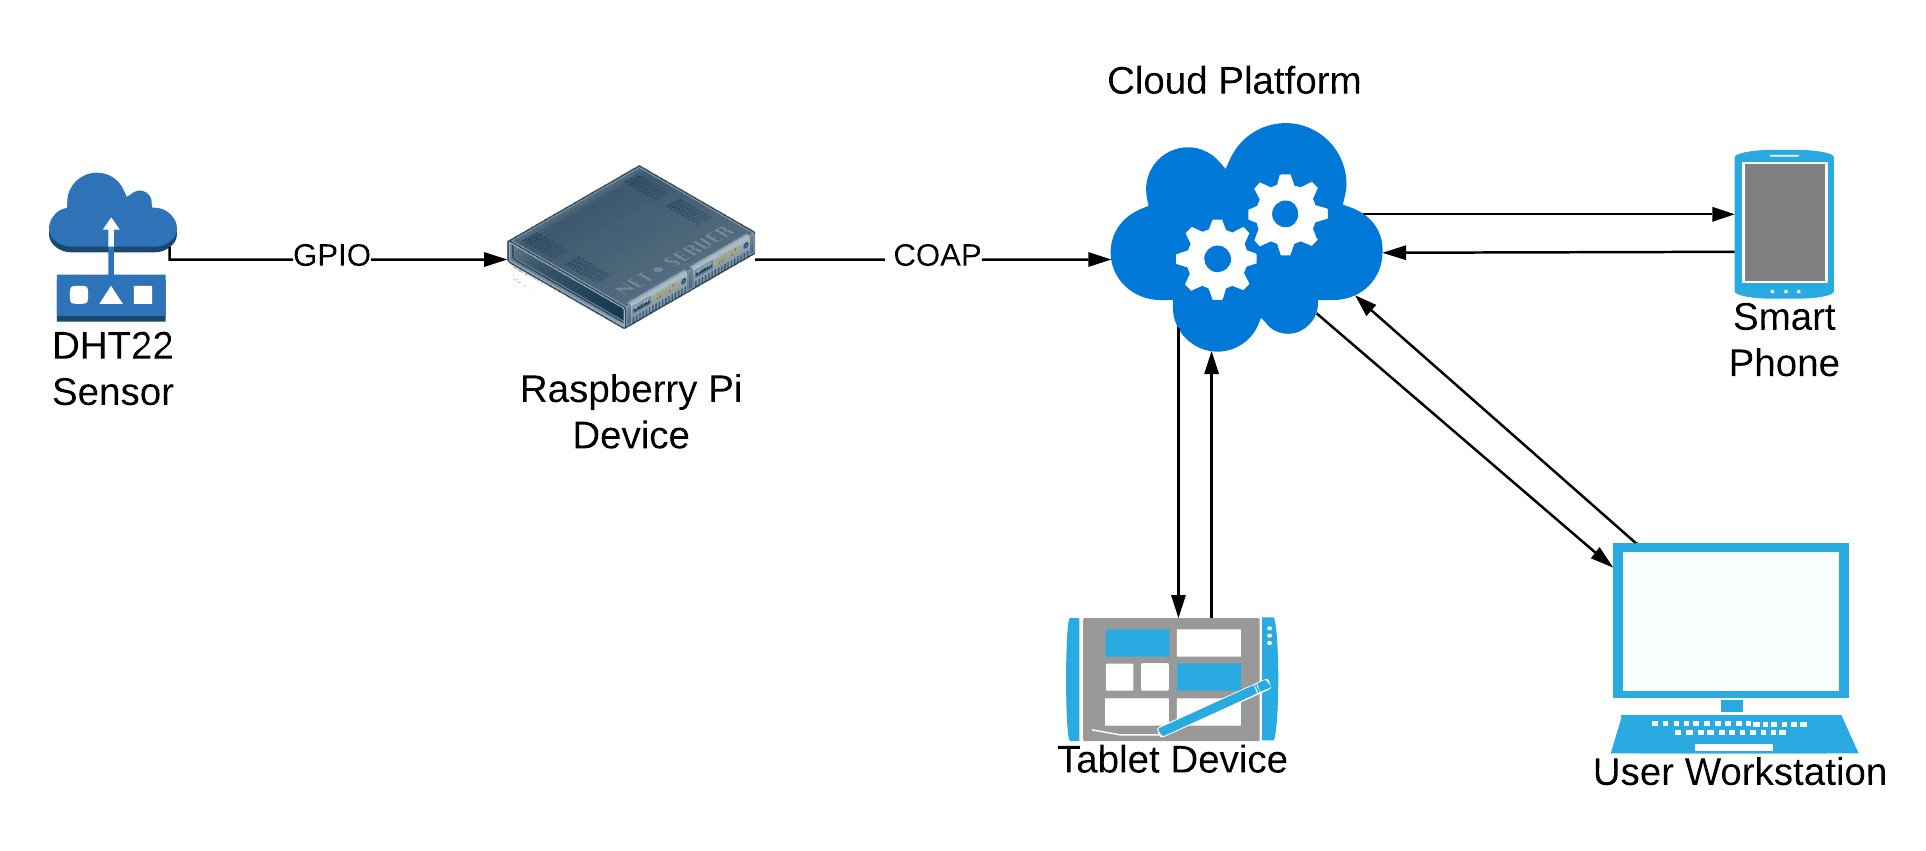
\includegraphics[width=\imageWidth\textwidth]{assets/Project_Framework.png}
    \caption{\label{fig:coap_iot_architecture} \gls{coap}-based \gls{iot} Architecture.}
\end{figure}

The system shall consist of four main elements: the sensor, the \gls{rpi}, 
\gls{coap} and the cloud platform.
The sensor will collect the data and pass this to the \gls{rpi}. 
The \gls{rpi} will then be responsible for manipulating
the data into a suitable format for transmission via \gls{coap}. 
The implementation of \gls{coap} will communicate with
the cloud platform. The cloud platform will store the data, 
allowing access to users.
The parts of the system are explained below:

\begin{figure}[H]
    \centering
   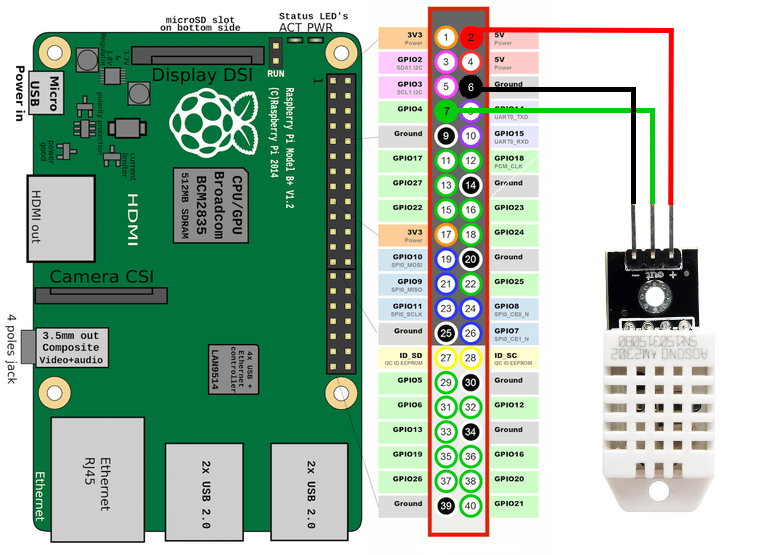
\includegraphics[width=\imageWidth\textwidth]{assets/rpi_wiring.png}
    \caption{\label{fig:rpi_wiring} Wiring diagram for connecting the DHT22 sensor to the \gls{rpi}.}
\end{figure}

\begin{description}
    \item[Sensors] 
    The DHT22/AM2302 digital relative temperature and humidity 
    sensor will be used to collect temperature and humidity data from the environment.
    The DHT22 has three pins: One for the 3.3--5.5V power, one for data output and
    one pin for neutral. The \gls{rpi} can connect to the DHT22 using the \gls{rpi}'s 
    \gls{gpio} ports to provide power, a ground connection and an output for the 
    DHT22's data, this connection is shown in \figref{fig:rpi_wiring}. The DHT 
    is capable of measuring temperatures in the range of -40 to 80 degrees celsius
    and reporting a relative humidity of between 0 to 100\% to an accuracy of $\pm2$\%.
    The largest negative to the DHT22 sensor is that it will only report new data
    once every two seconds, leading to reading being up to two seconds old.

    \item[Device]
    The Raspberry Pi 3 Model B is a Linux-based microcomputer.
    It includes built in WiFi, \gls{gpio} ports, a 1.2GHz Quad-Core processor,
    MicroSD card slot, memory, video/audio outputs, Ethernet port, and power source 
    \citep{pi_model_2018}. 
    It uses a MicroSD memory card as a boot drive and runs a specialised 
    GNU/Linux distribution named Raspbian \citep{raspbian_raspbian_2018}. Although the \gls{rpi} can be attached
    to a monitor using the built in HDMI port and controlled with a USB mouse and
    keyboard, this study will connect to the \gls{rpi} using SSH. The \gls{rpi} 
    will run a Python script which will collect the data from the DHT22 sensor 
    and send it to the \gls{coap} endpoint in the cloud.

    \item[Gateway]
    As this is a \gls{coap} based architecture and as such mirrors the workings
    of \gls{http} the gateway will be the local networks router. This will be 
    responsible for directing the \gls{coap} messages to the \gls{coap} endpoint
    identified by the cloud platforms \gls{uri}.

    \item[Cloud]
    This study will make use of an open source cloud platform, ThingsBoard.
    ThingsBoard is an \gls{iot} platform that allows the collection and 
    visualisation of data from \gls{iot} devices, connection from \gls{iot} devices
    using \gls{mqtt}, \gls{coap} or \gls{http}, the definition of rules to validate
    incoming data among other features. The \gls{rpi} will use the \gls{uri} 
    provided by the ThingsBoard \gls{coap} \gls{api} to send the sensor data to.
    Once ThingsBoard receives the sensor data it will update a dashboard which
    will show the temperature and humidity data provided by the sensor over time,
    this dashboard is displayed in \figref{fig:thingsboard_dashboard}.

\end{description}

The complete design of this system and how each component will interact
is illustrated in \figref{fig:coap_iot_architecture}.

The DHT22 sensor will connect to the \gls{rpi} using the \gls{rpi}'s on board 
\gls{gpio} ports as shown in \figref{fig:rpi_wiring}. 
The AdaFruit Python DHT library will be used in a Python script to get the 
sensor data from the DHT22 sensor.
The AdaFruit Python DHT library is a library that provides methods to interact 
with DHT sensors connected to the \gls{rpi}'s \gls{gpio} pins.
A \gls{coap} endpoint will need to be created on the \gls{rpi} in order to 
send the sensor data to the cloud. 
Using the CoAPthon Python library the script will create a \gls{coap} 
endpoint on the \gls{rpi}.
The CoAPthon library is a Python implementation of the \gls{coap} protocol.

\begin{center}
    \begin{algorithm}[htbp]
        \KwData{Temperature and humidity data from sensor}
        \KwResult{Sensor data sent to Cloud CoAP endpoint}
        initialisation\;
        define interval in seconds (DHT22 sensor interval is 2 seconds)\;
        \While{running}{
            get latest sensor data from DHT22 sensor\;
            \eIf{sensor data is returned}{
                format data into json object\;
                create CoAP Post message with cloud uri as destination\;
                send CoAP message\;
            }{
                wait interval time and continue\;
            }
        }
        \caption{\label{alg:get_send_data_alg}How to get data from sensor and send to cloud.}
    \end{algorithm}
\end{center}

This endpoint will act as an interface for the DHT22 sensor. 
At intervals the script will use the AdaFruit DHT library \citep{adafruit_adafruit_python_dht_2018} methods to retrieve 
the DHT22 sensor's current temperature and humidity readings. 
This data will then be formatted into \gls{json}
in order to be transmitted.
Then using the CoAPthon \citep{tanganelli_coapthon:_2015, tanganelli_coapthon3_2018} library a \gls{coap} 
message will be created with the sensors \gls{json} data as the payload. 
This loop will then repeat while the \gls{rpi} is active, this process is 
formalised in \algref{alg:get_send_data_alg}.
This message will then be sent over \gls{udp} to a \gls{coap} \gls{uri} 
hosted by the cloud platform as illustrated in \figref{fig:rpi_cloud_comms}.

\begin{figure}[H]
    \centering
    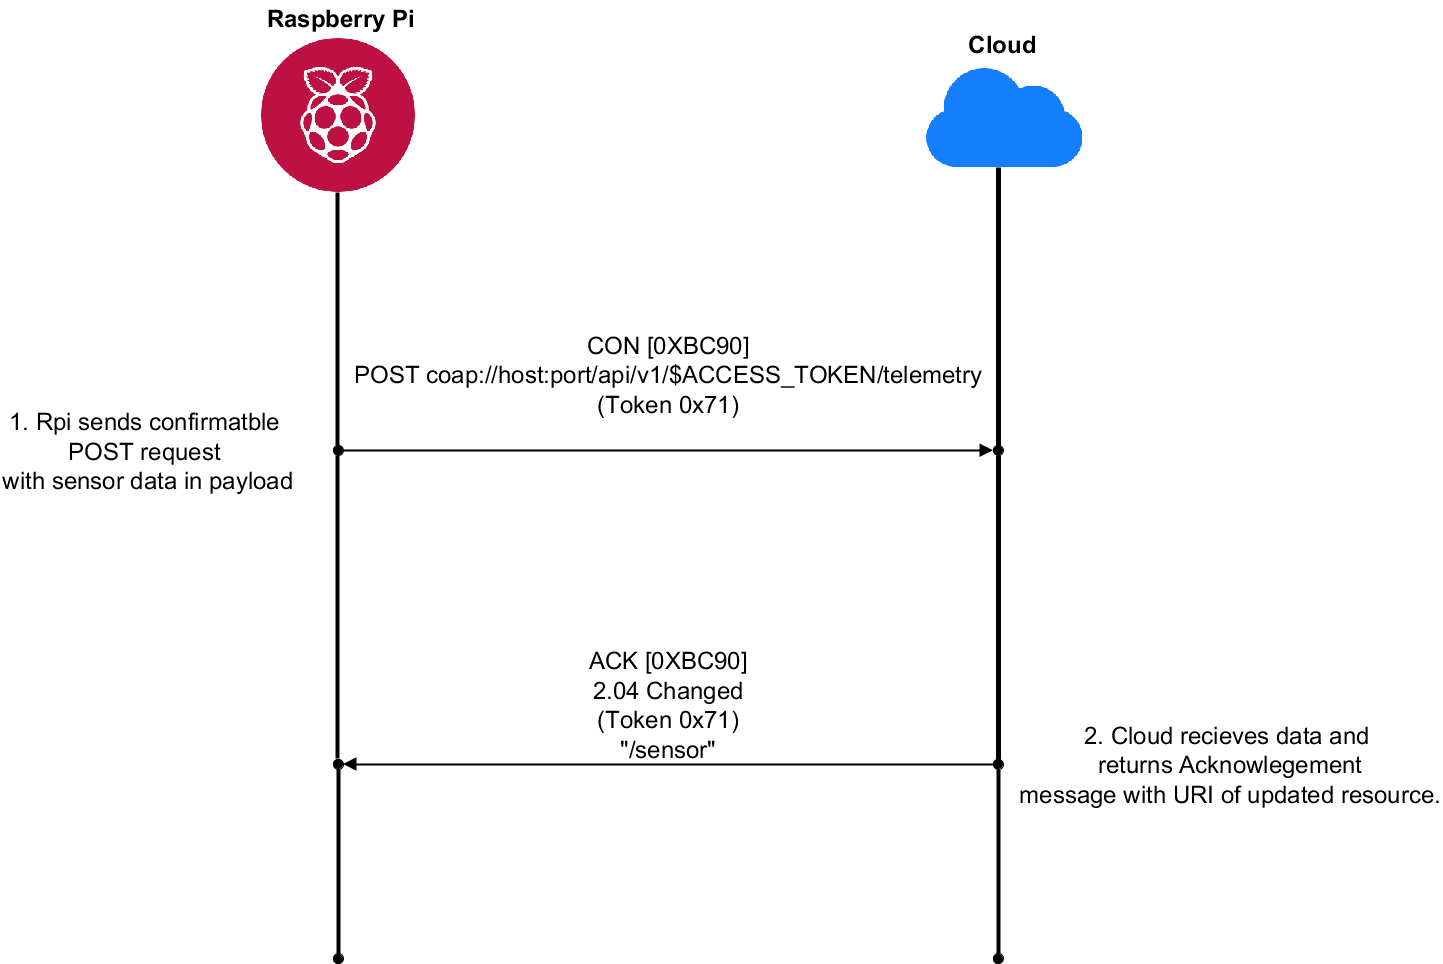
\includegraphics[width=\imageWidth\textwidth]{assets/rpi_cloud_communication.png}
    \caption{\label{fig:rpi_cloud_comms} Diagram showing the communication between \gls{rpi} and the Cloud.}
\end{figure}

The cloud's responsibility will be to receive the POST requests from the 
\gls{rpi} containing the \gls{json} data, format it and display it 
to the user, who will be accessing the cloud platform via \gls{http}. 
Once the ThingsBoard platform has received the request it should send an 
Acknowledgement message to the \gls{coap} endpoint, 
containing a 2.01 (Created) Response Code or a 2.04 (Changed) Response Code 
and the URI of the created / updated resource \citep{shelby_constrained_2014}. 